\documentclass{standalone}
\usepackage{tikz,color}
\begin{document}
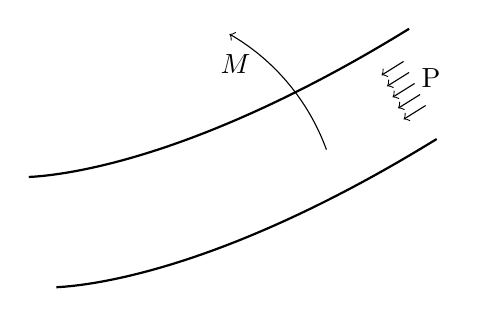
\begin{tikzpicture}[scale=0.7]


\draw [domain=1:70, samples=50, thick] plot( {0.1*\x}, {0.003*pow(\x,1.6)});
\draw [domain=1:70, samples=50, thick] plot( {0.1*\x-0.5}, {2+0.003*pow(\x,1.6)});

\draw [->] (5,2.5) arc [radius=4, start angle=20, end angle=60];
\node at (3.35,4.05) {$M$};

\draw[->] (6.4,4.1) to (6.0,3.85);
\draw[->] (6.5,3.9) to (6.1,3.65);
\draw[->] (6.6,3.7) to (6.2,3.45);
\draw[->] (6.7,3.5) to (6.3,3.25);
\draw[->] (6.8,3.3) to (6.4,3.05);

\node at (6.9,3.8) {P};

\end{tikzpicture}
\end{document}
